L'analyse statique de programmes est un sujet de recherche actif depuis
l'apparition de la science informatique.

\section{Méthodes syntaxiques}

L'analyse la plus simple consiste à traiter un programme comme du texte, et à y
rechercher des motifs dangereux. Ainsi, utiliser des outils comme \texttt{grep}
permet parfois de trouver un grand nombre de vulnérabilités~\cite{SpenderGrep}.

On peut continuer cette approche en recherchant des motifs mais en étant
sensible à la syntaxe et au flot de contrôle du programme. Cette notion de
\emph{semantic grep} est présente dans l'outil Coccinelle
\cite{coccinelle09,coccinelle11} \todo{lire coccinelle09} : on peut définir des
\emph{patches sémantiques} pour détecter ou modifier des constructions
particulières.

\section{Qualificateurs de types}

Dans le cas particulier des vulnérabilités liées à une mauvaise utilisation de
la mémoire, les développeurs du noyau Linux ont ajouté un système d'annotations
au code source. Un pointeur peut être décoré d'une annotation
\texttt{\_\_kernel} ou \texttt{\_\_user} selon s'il est sûr ou pas. Celle-ci
sont ignorées par le compilateur, mais un outil d'analyse statique ad-hoc nommé
Sparse \link{sparse} peut être utilisé pour détecter les cas les plus simples
d'erreurs.

Ce système d'annotations sur les types a été formalisé sous le nom de
\emph{qualificateurs de types} : chaque type peut être décoré d'un ensemble de
qualificateurs (à la manière de \texttt{const}), et des règles de typage
permettent d'établir des propriétés sur le programme. Ces analyses ont été
implantée dans l'outil CQual
\cite{pldi99,usenix01,pldi02,cquk-usenix04,toplas-quals}. \todo{lister les
applications}.

\section{Interprétation abstraite}

L'interprétation abstraite est une technique d'analyse générique qui permet de
simuler statiquement tous les comportements d'un programme Cousot
\cite{Cousot77,Cousot92-1}. Un exemple d'application est de calculer les bornes
de variations des variables pour s'assurer qu'aucun débordement de tableau n'est
possible. Cette technique est très puissante mais possède plusieurs
inconvénients. D'une part, pour réaliser une analyse interprocédurale il faut
partir d'un point en particulier du programme (comme la fonction \texttt{main}).
Cette hypothèse n'est pas facilement satisfaite dans un noyau de système
d'exploitation, qui possède de nombreux points d'entrée. D'autre part,
il est très difficile de faire passer à l'échelle un interpréteur abstrait
\cite{AstreeScale,coverityBillion}.

\begin{center}\rule{3in}{0.4pt}\end{center}

\begin{figure}%{{{
\centering
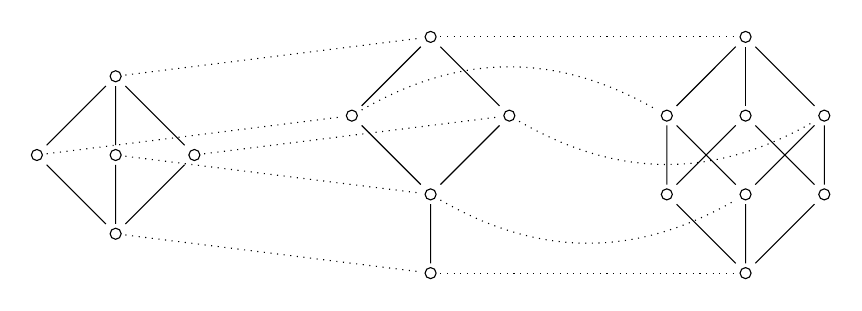
\begin{tikzpicture}
\node at (0,0) (lbase) {};
\path (lbase) +(0,0)  node (lb) {}
              +(-1,1) node (lm) {}
              +(0,1)  node (lz) {}
              +(1,1)  node (lp) {}
              +(0,2)  node (lt) {}
;
\draw (lb) -- (lm) -- (lt) -- (lz) -- (lb) -- (lp) -- (lt);

\node at (4,-0.5) (mbase) {};
\path (mbase) +(0,0)  node (mb)  {}
              +(0,1)  node (mz)  {}
              +(-1,2) node (mle) {}
              +(1,2)  node (mge) {}
              +(0,3)  node (mt)  {}
;
\draw (mb) -- (mz) -- (mle) -- (mt) -- (mge) -- (mz);

\node at (8,-0.5) (rbase) {};
\path (rbase) +(0,0)  node (rb)  {}
              +(-1,1) node (rlt) {}
              +(0,1)  node (rz)  {}
              +(1,1)  node (rgt) {}
              +(-1,2) node (rle) {}
              +(0,2)  node (rnz) {}
              +(1,2)  node (rge) {}
              +(0,3)  node (rt)  {}
;
\draw (rb) -- (rlt) -- (rle) -- (rt) -- (rge) -- (rgt) -- (rb) -- (rz) -- (rge);
\draw (rlt) -- (rnz) -- (rgt);
\draw (rz) -- (rle);
\draw (rnz) -- (rt);

\foreach \x in {lm,lz,lp,lb,lt,mb,mle,mz,mge,mt,rb,rlt,rz,rgt,rle,rnz,rge,rt}
  {\draw (\x) circle (2pt);}



\draw[dotted] (lb) -- (mb);
\draw[dotted] (lt) -- (mt);
\draw[dotted] (lm) -- (mle);
\draw[dotted] (lp) -- (mge);
\draw[dotted] (lz) -- (mz);

\draw[dotted] (mb) -- (rb);
\draw[dotted] (mt) -- (rt);
\draw[dotted] (mle) to [bend left=30] (rle);
\draw[dotted] (mge) to [bend right=30] (rge);
\draw[dotted] (mz)  to [bend right=30] (rz);

\end{tikzpicture}

\caption{Connexions de Galois}

\end{figure}%}}}

Les domaines les plus simples ne capturent aucune relation entre variables. Ce
sont des domaines non relationnels. On peut en citer quelques uns.

\paragraph{Le domaine des signes} capture uniquement le signe des variables
(figure~\ref{fig:dom-sig}).

\begin{figure}%{{{
\centering
\begin{tikzpicture}
\node at (1, 2) (t) {$\top$};
\node at (0, 1) (p) {$+$};
\node at (2, 1) (m) {$-$};
\node at (1, 0) (b) {$\bot$};
\draw (t) -- (p) -- (b);
\draw (t) -- (m) -- (b);
\end{tikzpicture}

\begin{align*}
\gamma~(+) = & \mathbb{R}^+ \\
\gamma~(-) = & \mathbb{R}^-
\end{align*}

\caption{Domaine des signes}
\label{fig:dom-sig}
\end{figure}%}}}

\paragraph{Le domaine des intervalles} retient les bornes de variations
extremales des variables (figure~\ref{fig:dom-intvl}).

\begin{figure} % {{{
\centering
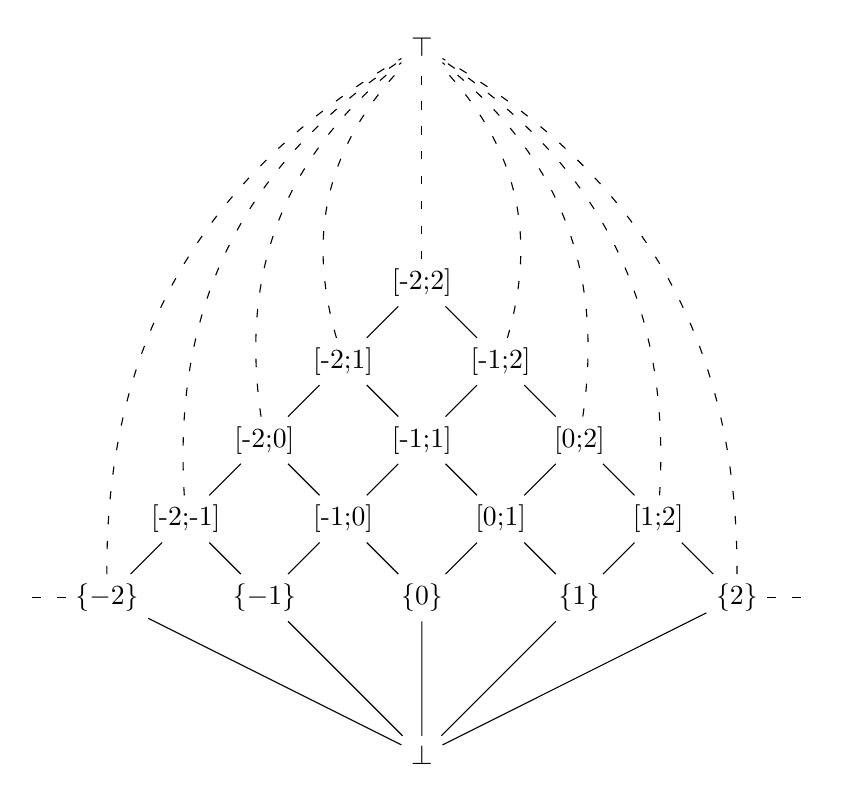
\begin{tikzpicture}
\node at (0,0)   (b)  {$\bot$};

\node at (-4,2) (cm2)   {$\{-2\}$};
\node at (-2,2) (cm1)   {$\{-1\}$};
\node at  (0,2)  (c0)   {$\{0\}$};
\node at  (2,2)  (c1)   {$\{1\}$};
\node at  (4,2)  (c2)   {$\{2\}$};

\node at (-3,3) (rm2m1) {[-2;-1]};
\node at (-1,3) (rm10)  {[-1;0]};
\node at  (1,3) (r01)   {[0;1]};
\node at  (3,3) (r12)   {[1;2]};

\node at (-2,4) (rm20)  {[-2;0]};
\node at  (0,4) (rm11)  {[-1;1]};
\node at  (2,4) (r02)   {[0;2]};

\node at (-1,5) (rm21)  {[-2;1]};
\node at  (1,5) (rm12)  {[-1;2]};

\node at  (0,6) (rm22)  {[-2;2]};

\node at  (0,9) (t)  {$\top$};

\draw (b) -- (cm2) -- (rm2m1) -- (rm20) -- (rm21) -- (rm22);
\draw (b) -- (cm1) -- (rm10) -- (rm11) -- (rm12);
\draw (b) -- (c0) -- (r01) -- (r02);
\draw (b) -- (c1) -- (r12);
\draw (b) -- (c2);

\draw (c2) -- (r12) -- (r02) -- (rm12) -- (rm22);
\draw (c1) -- (r01) -- (rm11) -- (rm21);
\draw (c0) -- (rm10) -- (rm20);
\draw (cm1) -- (rm2m1);

\draw[loosely dashed] (cm2)   to [bend left=30] (t);
\draw[loosely dashed] (rm2m1) to [bend left=30] (t);
\draw[loosely dashed] (rm20)  to [bend left=30] (t);
\draw[loosely dashed] (rm21)  to [bend left=30] (t);

\draw[loosely dashed] (rm22)  to (t);

\draw[loosely dashed] (rm12)   to [bend right=30] (t);
\draw[loosely dashed] (r02)   to [bend right=30] (t);
\draw[loosely dashed] (r12)   to [bend right=30] (t);
\draw[loosely dashed] (c2)    to [bend right=30] (t);

\draw[loosely dashed] (cm2) -- +(-1,0);
\draw[loosely dashed] (c2)  -- +(1,0);

\end{tikzpicture}

\caption{Domaine des intervalles}
\label{fig:dom-intvl}
\end{figure} % }}}

Lorsque plusieurs variables sont analysées en même temps, utiliser de tels
domaines revient à considérer un produit cartésien d'ensembles :

\begin{center}
  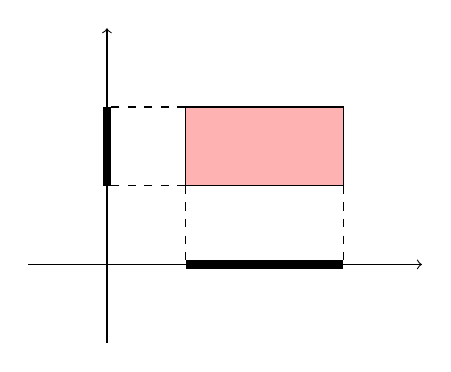
\begin{tikzpicture}
  \draw[->] (0,-1) -- (0,3);
  \draw[->] (-1,0) -- (4,0);

  \draw[fill=red!30] (1,1) rectangle (3,2);

  \draw[dashed] (3,1) -- (3,0);
  \draw[dashed] (1,1) -- (1,0);

  \draw[dashed] (1,2) -- (0,2);
  \draw[dashed] (1,1) -- (0,1);

  \draw[line width=3pt] (0,1) -- (0,2);
  \draw[line width=3pt] (3,0) -- (1,0);

  \end{tikzpicture}
\end{center}

Cela revient à oublier les relations entre les variables. Des domaines abstraits
plus précis permettent de retenir celles-ci. Pour ce faire, il faut modéliser
l'ensemble des valeurs des variables comme un tout.

\paragraph{Le domaines des polyèdres} est historiquement l'un des premiers
domaines relationnels. Il permet de retenir tous les invariants affines entre
fonctions (figure~\ref{fig:dom-poly}).

\begin{figure}%{{{
  \centering

  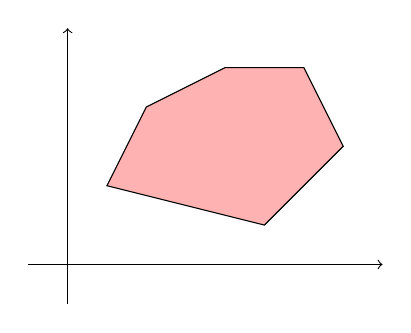
\begin{tikzpicture}[scale=0.5]
  \draw[->] (0,-1) -- (0,6);
  \draw[->] (-1,0) -- (8,0);

  \draw[fill=red!30] (1,2) -- (2,4) -- (4,5) -- (6,5) -- (7,3) -- (5,1) -- cycle;

  \end{tikzpicture}

  \[
  \vec{x} \in \mathcal{P}(A,B) \iff A \vec{x} \le B
  \]

\caption{Domaine des polyèdres}
\label{fig:dom-poly}

\end{figure}%}}}

\paragraph{Le domaine des zones} permet de représenter des relations affines de
forme $v_i - v_j \le c$ (figure~\ref{fig:dom-zones}).

\begin{figure}%{{{
  \centering
  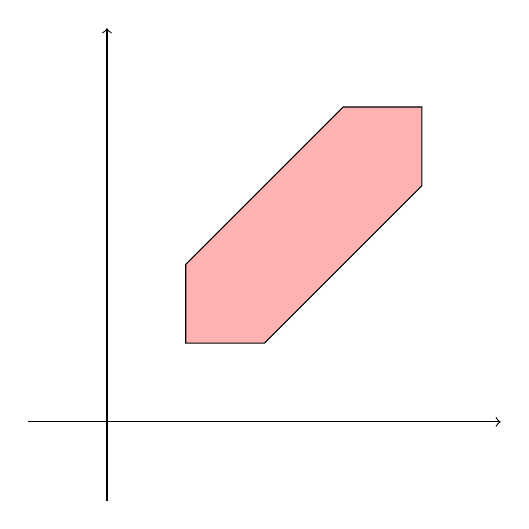
\begin{tikzpicture}
  \draw[->] (0,-1) -- (0,5);
  \draw[->] (-1,0) -- (5,0);

  \draw[fill=red!30] (1,2) -- (3,4) -- (4,4) -- (4,3) -- (2,1) -- (1,1) -- cycle;

  \end{tikzpicture}

  \caption{Domaine des zones}
  \label{fig:dom-zones}
\end{figure}%}}}

\paragraph{Le domaine des octogones} est un compromis entre les polyèdres et les
zones. Il permet de représenter les relations $\pm v_i \pm v_j \le c$
(figure~\ref{fig:dom-octo}).

\begin{figure}%{{{
  \centering
  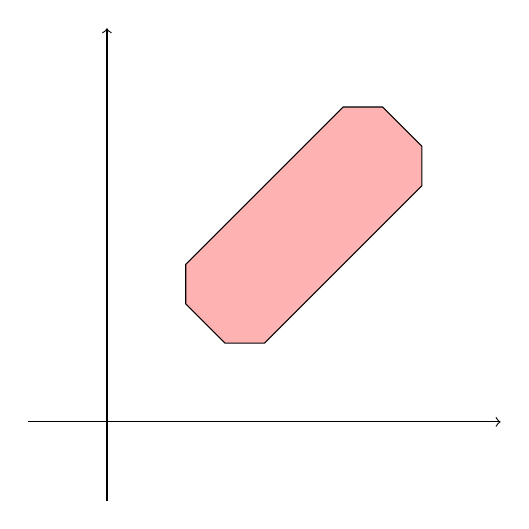
\begin{tikzpicture}
  \draw[->] (0,-1) -- (0,5);
  \draw[->] (-1,0) -- (5,0);

  \draw[fill=red!30] (1,1.5) -- (1,2) -- (3,4) -- (3.5,4) -- (4,3.5) -- (4,3) -- (2,1) -- (1.5,1) -- cycle;

  \end{tikzpicture}

  \caption{Domaine des octaèdres}
  \label{fig:dom-octo}
\end{figure}%}}}

\section{Typage}

L'approche par typage, plus légère, est séduisante. Pour les différents enjeux
des systèmes de types statiques, on pourra se référer à~\cite{TAPL}. Il est
possible d'encoder ce genre de propriétés dans un sytème de types, cf.
\cite{lightweight-static-capabilities} et \cite{LZ06a}.

\section{Logique de Hoare}

Pour raisonner sur un programme, on peut écrire les invariants qui sont vérifiés
à un point donné du programme. Ce sont des propositions écrits dans une logique
$\mathcal{L}$.

On peut aller plus loin que les simples types et utiliser un langage de contrats:
chaque fonction est annotée par des pré- et post-conditions sur la
mémoire.

\begin{itemize}
\item TODO relire \cite{cssv}
\item TODO citer Hoare\cite{hoare}
\item TODO citer Floyd\cite{FloydMeaning}
\item TODO citer C\# Contract (Rustan Leino)\cite{krml136}
\end{itemize}

Chaque instruction (ou \emph{commande}) $c$ est annotée d'une précondition $P$
et d'une postcondition $Q$, ce que l'on note :

\def\hoare#1#2#3{\ensuremath{\{#1\}~#2~\{#3\}}}

\[
\hoare{P}{c}{Q}
\]

En plus des règles de $\mathcal{L}$, des règles d'inférence traduisent la
sémantique du programme ; par exemple la règle de composition est :

\begin{mathpar}
  \irule{Hoare-Seq}
    { \hoare{P}{c_1}{Q} \\
      \hoare{Q}{c_2}{R}
    }{
      \hoare{P}{c_1;c_2}{R}.
    }
\end{mathpar}

Les préconditions peuvent être renforcées et les postconditions relaxées :
\begin{mathpar}
  \irule{Hoare-Consequence}
    { \vDash_{\mathcal{L}} P  ⇒ P' \\
      \hoare{P}{c}{Q} \\
      \vDash_{\mathcal{L}} Q' ⇒ Q
    }
    { \hoare{P'}{c}{Q'} }
\end{mathpar}

Il est alors possible d'annoter le programme avec ses invariants formalisés de
manière explicite dans $\mathcal{L}$. Ceux-ci seront vérifiés à la compilation.

\section{Analyse dynamique}

Du côté de l'analyse dynamique, \cite{oakland10}\todo{et Perl ?}.

\section{Analyse de flot}

Ce que nous voulons vérifier peut être vue comme une propriété de flot. Un
\emph{survey} des problèmes et techniques existantes peut être trouvé
dans~\cite{sm-jsac03}.

\wip{}

Interprétation Abstraite :
    widening \cite{granger},
    CGS \cite{cgs},
    Astrée : presentation\cite{Astree04,Astree05},

\section{Divers}

Divers : Taint sequences \cite{mdv10},

Frama-C ?

CCurred ?
